% LLNCS macro package for Springer Computer Science

\documentclass[runningheads]{llncs}
%
%
% Packages
%
\usepackage[bookmarks,hidelinks]{hyperref}
%
\usepackage{graphicx}
\usepackage{subfigure}
%
\usepackage{amsmath}
%
\usepackage[T1]{fontenc}
%\usepackage[spanish]{babel}
\usepackage[utf8]{inputenc}
%
\graphicspath{{img/}}

%
% Personal Commands
%
\newcommand{\refcruzada}[2]{\hyperref[#2]{#1~\ref{#2}}}

\newcommand{\comment}[1]{}

\newcommand{\addfigure}[2]{\begin{figure}
                               \includegraphics[scale=0.5]{#1} \centering \caption{#2} \label{fig:1}
\end{figure}}

% Used for displaying a sample figure. If possible, figure files should
% be included in EPS format.
%
% If you use the hyperref package, please uncomment the following line
% to display URLs in blue roman font according to Springer's eBook style:
% \renewcommand\UrlFont{\color{blue}\rmfamily}
%
%
\begin{document}
    %
    \title{Contribution Title\thanks{Trabajo desarrollado como proyecto final de la asignatura \textit{Agentes inteligentes y sistemas multiagente} del Máster Universitario en Inteligencia Artificial de la Universidad Politécnica de Madrid}}
    %
    %\titlerunning{Abbreviated paper title}
    % If the paper title is too long for the running head, you can set
    % an abbreviated paper title here
    %
    \author{Sergio Flórez Vallina}
    %

    % First names are abbreviated in the running head.
    % If there are more than two authors, 'et al.' is used.
    %
    \institute{Universidad Politécnica de Madrid, España\\
    \email{s.florez@alumnos.upm.es}\\
    }
    %
    \maketitle              % typeset the header of the contribution
    %
    \begin{abstract}
        The abstract should briefly summarize the contents of the paper in
        150--250 words.

        \keywords{First keyword  \and Second keyword \and Another keyword.}
    \end{abstract}
    %
    %
    %

    \section{Introducción}
    En los últimos años se ha observado que existen diversos problemas cuya naturaleza requiere de un enfoque multi-agente, pues un único agente no es capaz de resolverlos.
    Utilizando la Inteligencia Colectiva (CI), ya sea mediante una comunicación directa o indirecta entre los agentes, se han podido resolver problemas tanto en el ámbito de la robótica, tales como la planificación de rutas o construcción de estructuras complejas \cite{collectiveConstruction}, así como en el ámbito de la optimización, esto es, de encontrar la mejor solución --o al menos, una de buena calidad-- para un problema dado.
    En este artículo, analizaremos un posible sistema multiagente propuesto inicialmente en ~\cite{initialPaper}  con el objetivo de hallar la posición óptima de un espacio de búsqueda y su comportamiento frente a obstáculos físicos.
    La descripción del problema y las técnicas empleadas para su solución se encuentra en el \refcruzada{Apartado}{sec:descripcion}, y los resultados experimentales y el ajuste paramétrico en el \refcruzada{Apartado}{sec:}. %TODO poner referencias!!

    \section{Descripción del problema}
    \label{sec:descripcion}
    Tal y como se ha introducido anteriormente, el problema a resolver se basa en realizar una búsqueda dentro de un espacio bidimensional limitado a un cierto tamaño. Trataremos de maximizar una función conocida $f(x,y)$, sujeta a las restricciones de espacio impuestas inicialmente, es decir, al tamaño del mapa por el que se moverán los agentes.
    Para su desarrollo, se ha utilizado como base la técnica propuesta por ~\cite{initialPaper}, sin embargo ésta no contempla el uso de obstáculos --ciertas posiciones del espacio que no pueden ser traspasados por el robot-- dentro del espacio de búsqueda, por lo que se ha extendido y adaptado.
    En el \refcruzada{Apartado}{3} se muestran algunos ejemplos que lo ilustran, utilizando tanto obstáculos como diferentes funciones objetivo. %TODO referencias


    \subsection{El espacio de búsqueda}
    La representación propuesta en ~\cite{initialPaper} consiste en discretizar el espacio de búsqueda en forma de una cuadrícula (\textit{grid}). Ésta es una de las formas clásicas más sencillas de representar un espacio de búsqueda, sin embargo, tal y como se apuntan en ~\cite{AIRobotics}, este tipo de representación conlleva a una \textit{digitalización} o discretización del espacio con una cierta granularidad dada. A mayor granularidad, mayor fidelidad en la representación del espacio. En el artículo original, se utiliza una única granularidad sobre una cuadrícula $10 \times 10$. En el \refcruzada{Apartado}{3} se prueban diferentes tamaños. %TODO es esto cierto??

    Podemos considerar el espacio de búsqueda a efectos prácticos, como una colina tridimensional donde la tercera dimensión representa la intensidad de una señal que sigue una función (no necesariamente lineal). La finalidad del sistema es que los agentes colaboren para alcanzar el punto más álgido.

    \subsection{La estrategia de resolución}

    Los agentes llevan a cabo movimientos sencillos empleando información en común entre sí, pero de forma indirecta, a través del medio. Éste tipo de soluciones reciben el nombre de sistemas basados en \textit{estigmergia}~\cite{stigmergy}.
    
    % lo muevo como parrafo para evitar un bad-box
    Como buen sistema multiagente, podemos observar una capacidad de auto-organización (\textit{self-organization}), mediante el cual emerge un comportamiento de características más complejas, que en este caso consisten en localizar y converger a un lugar concreto del mapa.

    En este enfoque, los agentes se moverán libremente por el espacio, sin limitarse a la cuadrícula, y depositarán en las respectivas celdas sobre las que se encuentre, una información dada que llamaremos feromonas, que estarán representadas mediante un vector cuya dirección y sentido sea la más prometedora del espacio y cuyo módulo será proporcional a la mejora que aporta dicho movimiento al valor de la función objetivo. El cálculo de dichas feromonas se lleva a cabo siguiendo una estrategia basada en un sistema PSO (\textit{Particle Swarm Optimization})~\cite{PSO} combinado con información heurística dada por la función objetivo según las formulas descritas en el articulo \cite{initialPaper}, mientras que el depósito y combinación de las feromonas en el entorno se basa en este caso en los sistemas ACO (\textit{Ant Colony Optimization})~\cite{ACO}.
    
    Nótese que la dirección vendrá dada por la posición hacia la que se está moviendo el robot, mientras que el sentido y el módulo del mismo dependerá de la función objetivo de forma directamente proporcional a ésta.

    Por último, para poder evitar los obstáculos, en caso de que el agente no sea capaz de mejorar su mejor solución local tras un número máximo de iteraciones, se generará una nueva velocidad con dirección y sentido arbitrario, y con módulo $V_{max}$, la velocidad máxima posible de los agentes. En caso de no poder sortear el obstáculo, se trata durante otro cierto número de iteraciones, de rotar el vector velocidad generado anteriormente una cantidad de grados, en este caso de $10$ (véase~\cite{referencedPaper}).


    \section{Resultados experimentales}

    % TODO: poner tablas con los valores de todos los parámetros del sistema


    \subsection{Variaciones en la función objetivo}
    En el artículo original \cite{initialPaper} únicamente se utilizaba una función lineal, cuyo punto máximo se hallaba en el $(8,8)$ de una cuadrícula de $10\times10$, ésto es así debido a que el enfoque de sus autores no era la optimización de la misma, sino una futura implementación a nivel físico, donde la función objetivo sería implementada mediante una señal (acústica o lumínica). Para analizar el potencial de éste sistema, se han probado algunas funciones de optimización conocidas, recopiladas en \cite{WebFuncionesOptimizacion}.

    \subsubsection{Función de Ackley} Propuesta en \cite{AckleyFunction} se define como
    \[ f(x,y)=-20 \cdot exp[-0.2 \cdot \sqrt{0.5 \cdot (x^2 + y^2)}] - exp[0.5 ( \cos(2 \pi x)
    + \cos(2 \pi y))] + e + 20)\]
    Al estar pensada para minimización y definida en el intervalo $[-5,5]$, consideramos la función $f'(x,y)=(-1)\cdot f(x-5, y-5)$. Se trata de una función no convexa, con una gran cantidad de máximos locales, como puede apreciarse en la \refcruzada{Fig.}{fig:2:b}, siendo el máximo absoluto el punto $(5,5)$.
    
    \begin{figure}[htbp]
    	\centering
    	\subfigure[Gráfica sobre 3 ejes]{
    		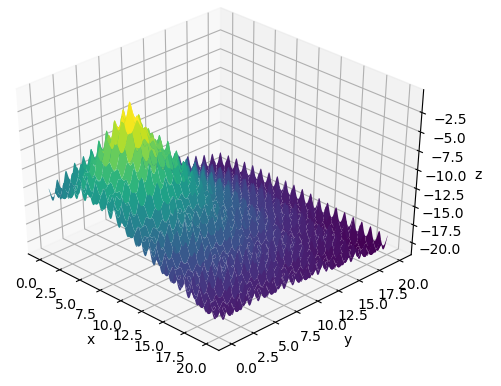
\includegraphics[width=0.4\textwidth]{graficas_ackley}
    		\label{fig:2:a}
    	}
    	\subfigure[Curvas de nivel]{
    		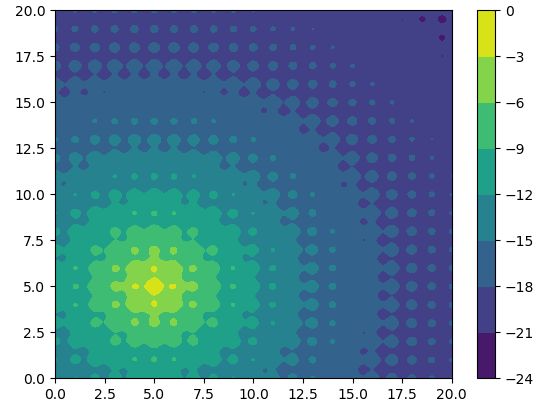
\includegraphics[width=0.5\textwidth]{graficas_ackley_contorno}
    		\label{fig:2:b}
    	}
    	\caption{Representación de la función Ackley modificada para $x,y\in[0,20]$}
    \end{figure}
    
    Los resultados tras 1\,300 iteraciones es el de la \refcruzada{Fig.}{fig:3}, como puede verse, se produce una convergencia casi total hace el punto $(5,5)$, sin embargo el mapa de feromonas construido no es útil, pues prácticamente todos los valores son de módulo cero.

    \begin{figure}[htbp]
		\centering
		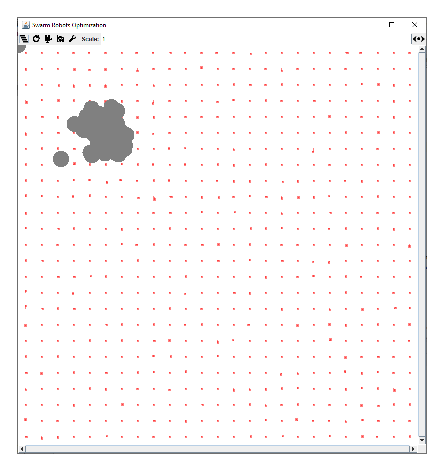
\includegraphics[width=0.5\textwidth]{Resultado_ackley}
		\label{fig:3}
		\caption{Resultados experimentales empleando la función Ackley}
	\end{figure}

    \subsubsection{Función de Himmelblau} Propuesta en \cite{HimmelblauFunction} se define para el caso de una maximización como
    \[  f(x,y)=-(x^2 + y - 11)^2 - (x + y^2 - 7)^2  \] 
    Contiene una meseta en la parte superior, por lo que no existe una única solución (ver \hyperref[fig:4]{Fig. 3}).
    En cuanto a los resultados obtenidos, mostrados en la \hyperref[fig:5]{Fig. 4}, el sistema no es capaz de converger, en su lugar, se forman 3 grupos de agentes en torno a los 4 posibles óptimos que tiene la función (ver \cite{WebFuncionesOptimizacion} para más información)


    \begin{figure}[htbp]
		\centering
		\subfigure[Gráfica sobre 3 ejes]{
			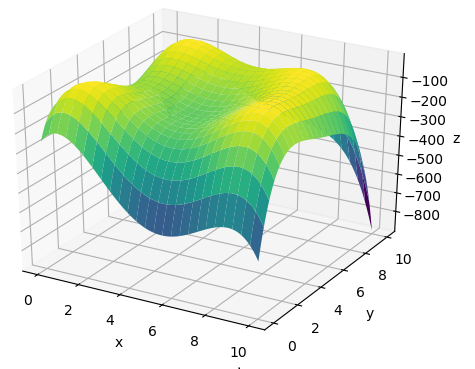
\includegraphics[width=0.4\textwidth]{graficas_himmelblau}
		}
		\subfigure[Curvas de nivel]{
			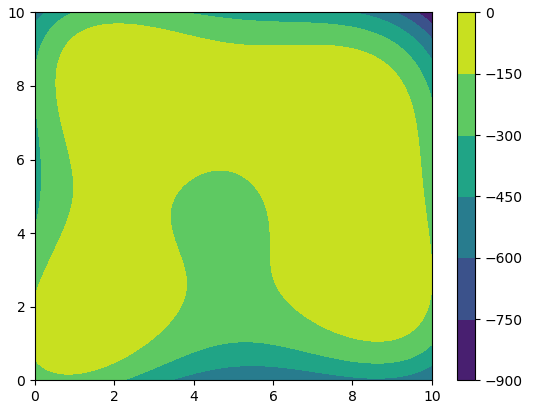
\includegraphics[width=0.5\textwidth]{graficas_himmelblau_contorno}
		}
		\label{fig:4}
		\caption{Representación de la función Himmelblau modificada para $x,y\in[0,10]$}
	\end{figure}

balbalblbalal

    \begin{figure}[htbp]
   	\centering
   	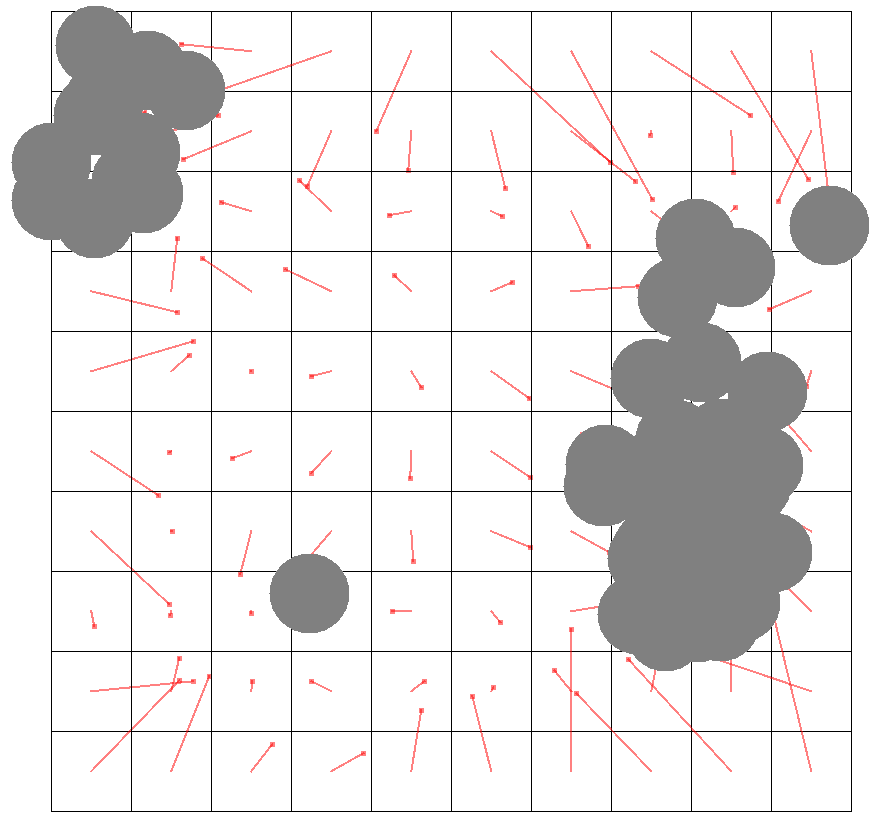
\includegraphics[width=0.5\textwidth]{Resultados_himmelblau_10x10}
   	\label{fig:5}
   	\caption{Resultados experimentales empleando la función Himmelblau sobre una cuadricula $10\times10$}
   \end{figure}

\comment{
    \subsubsection{Función Lineal}
    $f(x,y)=-(x-g_x)^2 - (y - g_y)^2 + 700$; con máximo en $(g_x,g_y)$
}
    \subsection{Pruebas con obstáculos}









    \comment{
    \section{First Section}
    \subsection{A Subsection Sample}
    Please note that the first paragraph of a section or subsection is
    not indented. The first paragraph that follows a table, figure,
    equation etc. does not need an indent, either.

    Subsequent paragraphs, however, are indented.

    \subsubsection{Sample Heading (Third Level)} Only two levels of
    headings should be numbered. Lower level headings remain unnumbered;
    they are formatted as run-in headings.

    \paragraph{Sample Heading (Fourth Level)}
    The contribution should contain no more than four levels of
    headings. Table~\ref{tab1} gives a summary of all heading levels.

    \begin{table}
        \caption{Table captions should be placed above the
        tables.}\label{tab1}
        \begin{tabular}{|l|l|l|}
            \hline
            Heading level & Example & Font size and style\\
            \hline
            Title (centered)  & {\Large\bfseries Lecture Notes}                 & 14 point, bold   \\
            1st-level heading & {\large\bfseries 1 Introduction}                 & 12 point, bold   \\
            2nd-level heading & {\bfseries 2.1 Printing Area}                     & 10 point, bold   \\
            3rd-level heading & {\bfseries Run-in Heading in Bold.} Text follows & 10 point, bold   \\
            4th-level heading & {\itshape Lowest Level Heading.} Text follows & 10 point, italic \\
            \hline
        \end{tabular}
    \end{table}


    \noindent Displayed equations are centered and set on a separate
    line.
    \begin{equation}
        x + y = z
    \end{equation}
    Please try to avoid rasterized images for line-art diagrams and
    schemas. Whenever possible, use vector graphics instead (see
    Fig.~\ref{fig1}).

    \begin{figure}
        \includegraphics[width=\textwidth]{fig1.eps}
        \caption{A figure caption is always placed below the illustration.
        Please note that short captions are centered, while long ones are
        justified by the macro package automatically.} \label{fig1}
    \end{figure}

    \begin{theorem}
        This is a sample theorem. The run-in heading is set in bold, while
        the following text appears in italics. Definitions, lemmas,
        propositions, and corollaries are styled the same way.
    \end{theorem}
    %
    % the environments 'definition', 'lemma', 'proposition', 'corollary',
    % 'remark', and 'example' are defined in the LLNCS documentclass as well.
    %
    \begin{proof}
        Proofs, examples, and remarks have the initial word in italics,
        while the following text appears in normal font.
    \end{proof}
    For citations of references, we prefer the use of square brackets
    and consecutive numbers. Citations using labels or the author/year
    convention are also acceptable. The following bibliography provides
    a sample reference list with entries for journal
    articles~\cite{ref_article1}, an LNCS chapter~\cite{ref_lncs1}, a
    book~\cite{ref_book1}, proceedings without editors~\cite{ref_proc1},
    and a homepage~\cite{ref_url1}. Multiple citations are grouped
    \cite{ref_article1,ref_lncs1,ref_book1},
    \cite{ref_article1,ref_book1,ref_proc1,ref_url1}.
    }
    %
    % ---- Bibliography ----
    %
    % BibTeX users should specify bibliography style 'splncs04'.
    % References will then be sorted and formatted in the correct style.
    %
    \bibliographystyle{splncs04}
    \bibliography{main}

\end{document}
